%%%%%%%%%%%%%%%%%%%%%%%%%%%%%%%%%%%%%%%%%%%%%%%%%%%%%%%%%%%%%%%%%%%%%%
% LaTeX Example: Project Report
%
% Source: http://www.howtotex.com
%
% Feel free to distribute this example, but please keep the referral
% to howtotex.com
% Date: March 2011 
% 
%%%%%%%%%%%%%%%%%%%%%%%%%%%%%%%%%%%%%%%%%%%%%%%%%%%%%%%%%%%%%%%%%%%%%%
% How to use writeLaTeX: 
%
% You edit the source code here on the left, and the preview on the
% right shows you the result within a few seconds.
%
% Bookmark this page and share the URL with your co-authors. They can
% edit at the same time!
%
% You can upload figures, bibliographies, custom classes and
% styles using the files menu.
%
% If you're new to LaTeX, the wikibook is a great place to start:
% http://en.wikibooks.org/wiki/LaTeX
%
%%%%%%%%%%%%%%%%%%%%%%%%%%%%%%%%%%%%%%%%%%%%%%%%%%%%%%%%%%%%%%%%%%%%%%
% Edit the title below to update the display in My Documents
%\title{Project Report}
%
%%% Preamble
\documentclass[paper=a4, fontsize=11pt]{scrartcl}
\usepackage[T1]{fontenc}
\usepackage{fourier}

\usepackage[english]{babel}															% English language/hyphenation
\usepackage[protrusion=true,expansion=true]{microtype}	
\usepackage{amsmath,amsfonts,amsthm} % Math packages
\usepackage[pdftex]{graphicx}	
\usepackage{url}
\usepackage[titletoc,title]{appendix}
\usepackage[options ]{algorithm2e}
\usepackage{listings}


%%% Custom sectioning
\usepackage{sectsty}
\allsectionsfont{\centering \normalfont\scshape}


%%% Custom headers/footers (fancyhdr package)
\usepackage{fancyhdr}
\pagestyle{fancyplain}
\fancyhead{}											% No page header
\fancyfoot[L]{}											% Empty 
\fancyfoot[C]{}											% Empty
\fancyfoot[R]{\thepage}									% Pagenumbering
\renewcommand{\headrulewidth}{0pt}			% Remove header underlines
\renewcommand{\footrulewidth}{0pt}				% Remove footer underlines
\setlength{\headheight}{13.6pt}


%%% Equation and float numbering
\numberwithin{equation}{section}		% Equationnumbering: section.eq#
\numberwithin{figure}{section}			% Figurenumbering: section.fig#
\numberwithin{table}{section}				% Tablenumbering: section.tab#


%%% Maketitle metadata
\newcommand{\horrule}[1]{\rule{\linewidth}{#1}} 	% Horizontal rule

\title{
		%\vspace{-1in} 	
		\usefont{OT1}{bch}{b}{n}
		\normalfont \normalsize \textsc{Braket Technologies Technical Report} \\ [25pt]
		\horrule{0.5pt} \\[0.4cm]
		\huge Bearing Angle Errors Due to Pipe Background \\
		\horrule{2pt} \\[0.5cm]
}
\author{
		\normalfont 								\normalsize
        Braket Technologies\\[-3pt]		\normalsize
        \today
}
\date{}


%%% Begin document
\begin{document}
\maketitle
\section{Introduction}
Scott.  Maybe you can write something in here that sets the context for this work.  The type of instrument used, the circumstances that triggered this work, etc.

\section{Illustrative Measurements}
The xxx instrument produces timeseries measurements consisting of a time-stamp, a bearing angle and a signal strength.  Fig. \ref{fig:sample_time_trace} shows one such measurement run.  The instrument is placed at a particular location within the pipe being measured.  While remaining at a fixed location in the pipe, the instrument rotates to capture measure signal the signal strength as a function of bearing.  After that location has been measured, the instrument stops rotating and is moved to a different location within the pipe where the process is repeated.

\par Although the time-series plots are useful for visualizing entire measurement runs, the signal dependence on bearing at a particular location is most useful and is shown in Fig. \ref{fig:sample_bearing_trace}


\begin{figure}[h!]
  \caption{A time-series from the XXX instrument taken during a calibration run. The interval between 0 and 120 seconds is taken at a fixed location in the pipe while rotating through different bearing angles.  Rotation is then stopped for the period between 120 and 220 seconds as the instrument is moved to a different pipe location.  This second location is then measured in the interval between 220 and 360 seconds.}
  \label{fig:sample_time_trace}
  \centering
  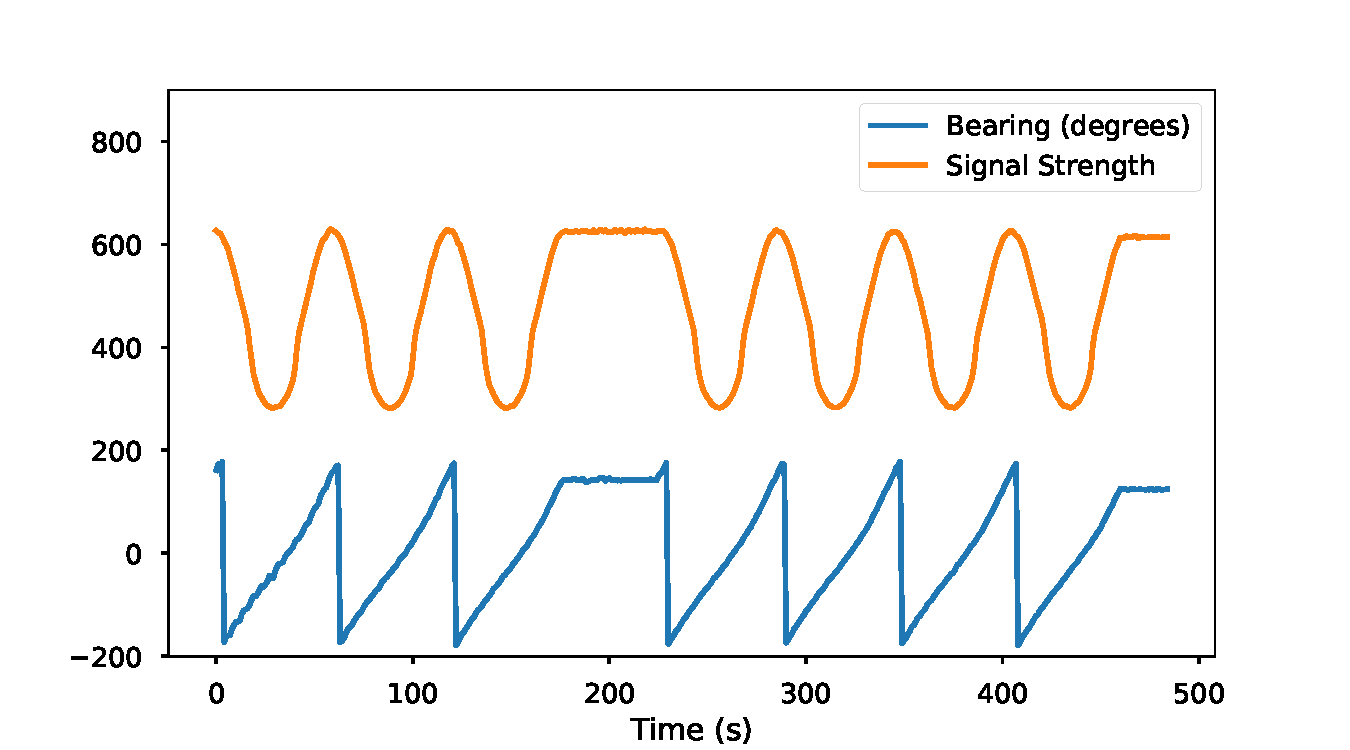
\includegraphics[width=1.0\textwidth]{figures/sample_time_trace.pdf}
\end{figure}

\begin{figure}[h!]
  \caption{These traces show how the presence of the cable alters the angular dependence of the signal strength.  The relative signal strengths, amplitude variations and phase of the resulting traces will depend on the details of the background and cable signals.}
  \label{fig:sample_bearing_trace}
  \centering
  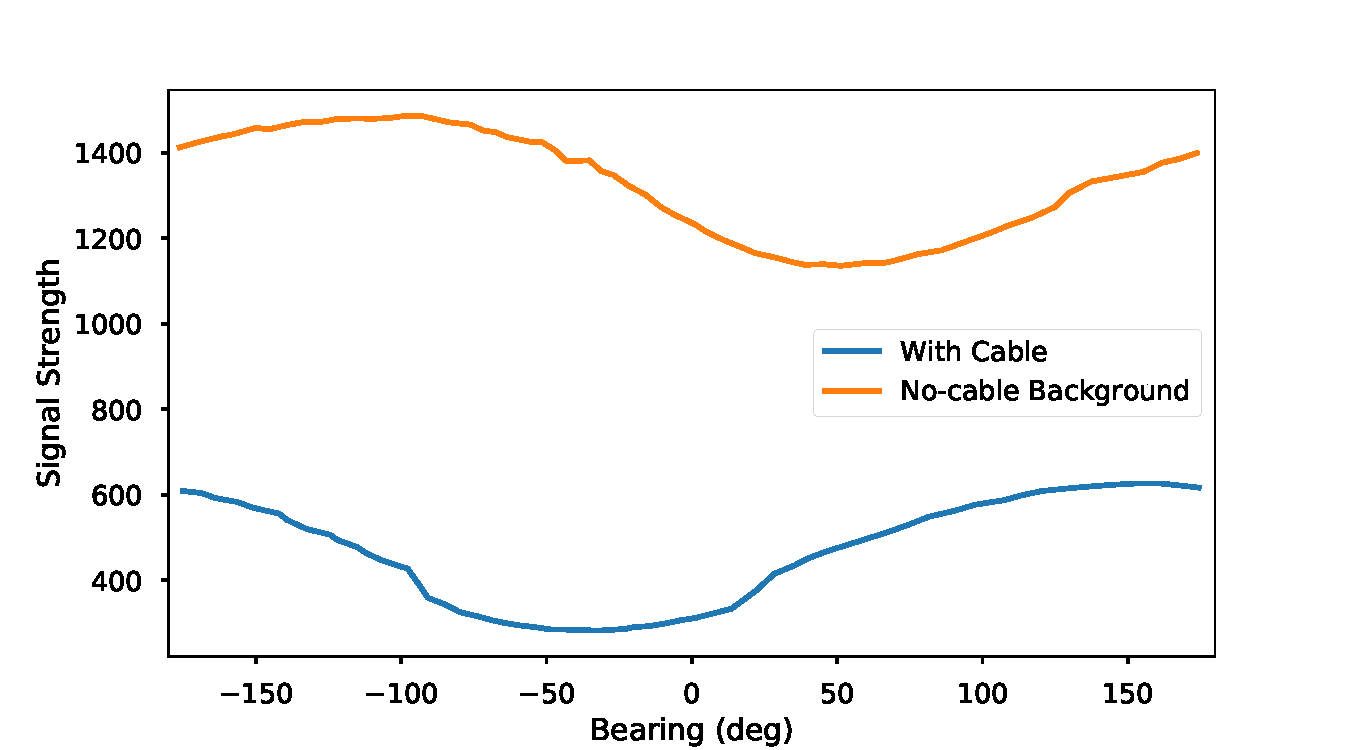
\includegraphics[width=1.0\textwidth]{figures/sample_bearing_trace.pdf}
\end{figure}

\section{Mathematical Model}
We model the bearing dependence of signal strength as simple sinusoidal functions of unknown amplitude and phase.  Although the curve shapes in Fig. \ref{fig:sample_bearing_trace} are not perfect fits, we find that the sinusoidal model captures the important relevant features.
\par In the absence of the cable, background signals are measured by the instrument.  These are thought to be dominated by imperfect centering within the pipe bore, but other effects include angular variations of the tube-wall properties.  When the cable is present, the angular asymmetry it introduces also creates a angular variation of the signal strength, which we again model with a sinusoidal function.  The total signal measured will be the sum of background and cable variations and are modeled by the equation
\begin{equation} \label{eq:trig_sig}
    s = C sin\left(\theta + \phi_1\right) + B sin\left(\theta + \phi_2\right),
\end{equation}
where
\begin{align}
        S &= \text{total signal amplitude} \\
        C &= \text{cable signal amplitude} \\
        B &= \text{background signal amplitude.}
\end{align}
This means that, for any measurement set our model requires us to specify four parameters: two amplitudes and two phases.  \par This problem becomes more intuitive if we use phasors to represent the two signals being added.


\section{Begin Examples}
And of course, this is just an example of how to do equations.  I'll keep it here as a template for working with equations below.
\begin{align} 
	\begin{split}
	(x+y)^3 	&= (x+y)^2(x+y)\\
					&=(x^2+2xy+y^2)(x+y)\\
					&=(x^3+2x^2y+xy^2) + (x^2y+2xy^2+y^3)\\
					&=x^3+3x^2y+3xy^2+y^3
	\end{split}					
\end{align}

\subsection{Example of a susection}
Subsection text with another equation.  And here is a figure.

\begin{align}
	A = 
	\begin{bmatrix}
	A_{11} & A_{21} \\
  	A_{21} & A_{22}
	\end{bmatrix}
\end{align}
And some more text. And maybe another figure.

\subsubsection{SubSub section}
More text here

\paragraph{Paragraph Header if you want it}
Some stuff in a paragragh.

\paragraph{}
See if this is a new paragraph.


\section{Lists}

\subsection{Example for list (3*itemize)}
\begin{itemize}
	\item First item in a list 
		\begin{itemize}
		\item First item in a list 
			\begin{itemize}
			\item First item in a list 
			\item Second item in a list 
			\end{itemize}
		\item Second item in a list 
		\end{itemize}
	\item Second item in a list 
\end{itemize}

\subsection{Example for list (enumerate)}
\begin{enumerate}
	\item First item in a list 
	\item Second item in a list 
	\item Third item in a list
\end{enumerate}


\begin{appendices}
\section{Estimating the Bearing Correction}
\subsection{The Bearing Correction}
The signal measured within the pipe will vary as a function of angle.  We can break down the source of this signal into two components.  The first component we will call the ``cable signal.''  This is the signal variation caused by the presence of the cable attached to the outside of the pipe.  The second component we will call the ``background signal,'' which arises from all other sources of angular asymmetry in the system.  This is thought to be dominated by imperfect centering of the instrument within the pipe.

\par We model both the background and cable signals as if they were sinusoidal function.  Figure \ref{fig:sigs_vs_bearing} shows a model we will use as an example for describing our analysis.  In this model, the background signal is one quarter the amplitude of the cable signal and it is offset in angle by 135 degrees.  The instrument will measure the sum of these two signals, which, of course, will have a different amplitude and phase than either of is constituent signals.

\begin{figure}
  \caption{An Example Model.  The background signal is one quarter the amplitude of the cable signal, and has a 135 degree offset in bearing.}
  \label{fig:sigs_vs_bearing}
  \centering
  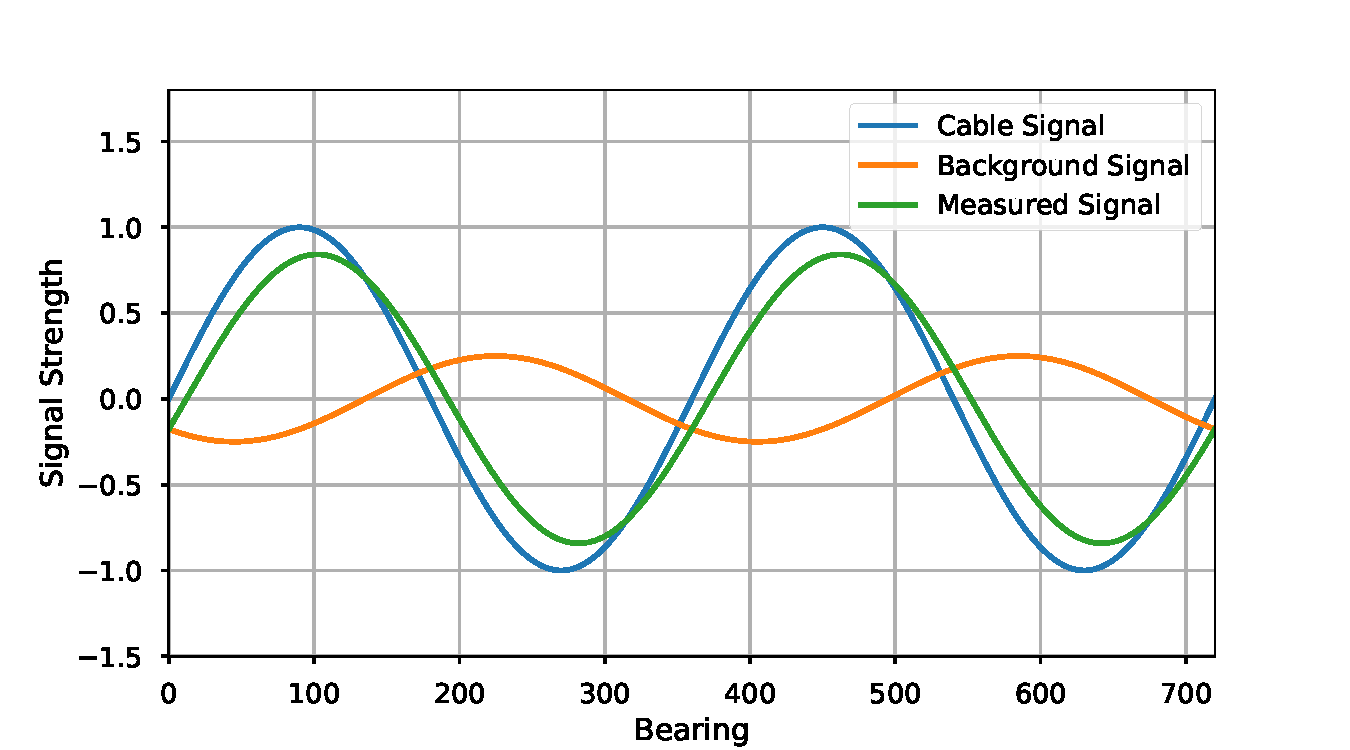
\includegraphics[width=1.0\textwidth]{figures/sigs_vs_bearing.pdf}
\end{figure}

\begin{figure}
  \caption{
  The phasor representation of the example model from Figure \ref{fig:sigs_vs_bearing}. $s$ is the measured cable signal, $b$ the background phasor and $m$ the measured phasor.  The value we really care about is $\theta$, the angle between the measured and cable signals.  Note that we can only determine the magnitude of the angle, but not the sign.  The phasor relationships shown in solids lines are indistinguishable from those shown by the dashed lines.  This model provides no information for distinguishing between the $\pm\theta$ solutions}
  \label{fig:phasor_base}
  \centering
  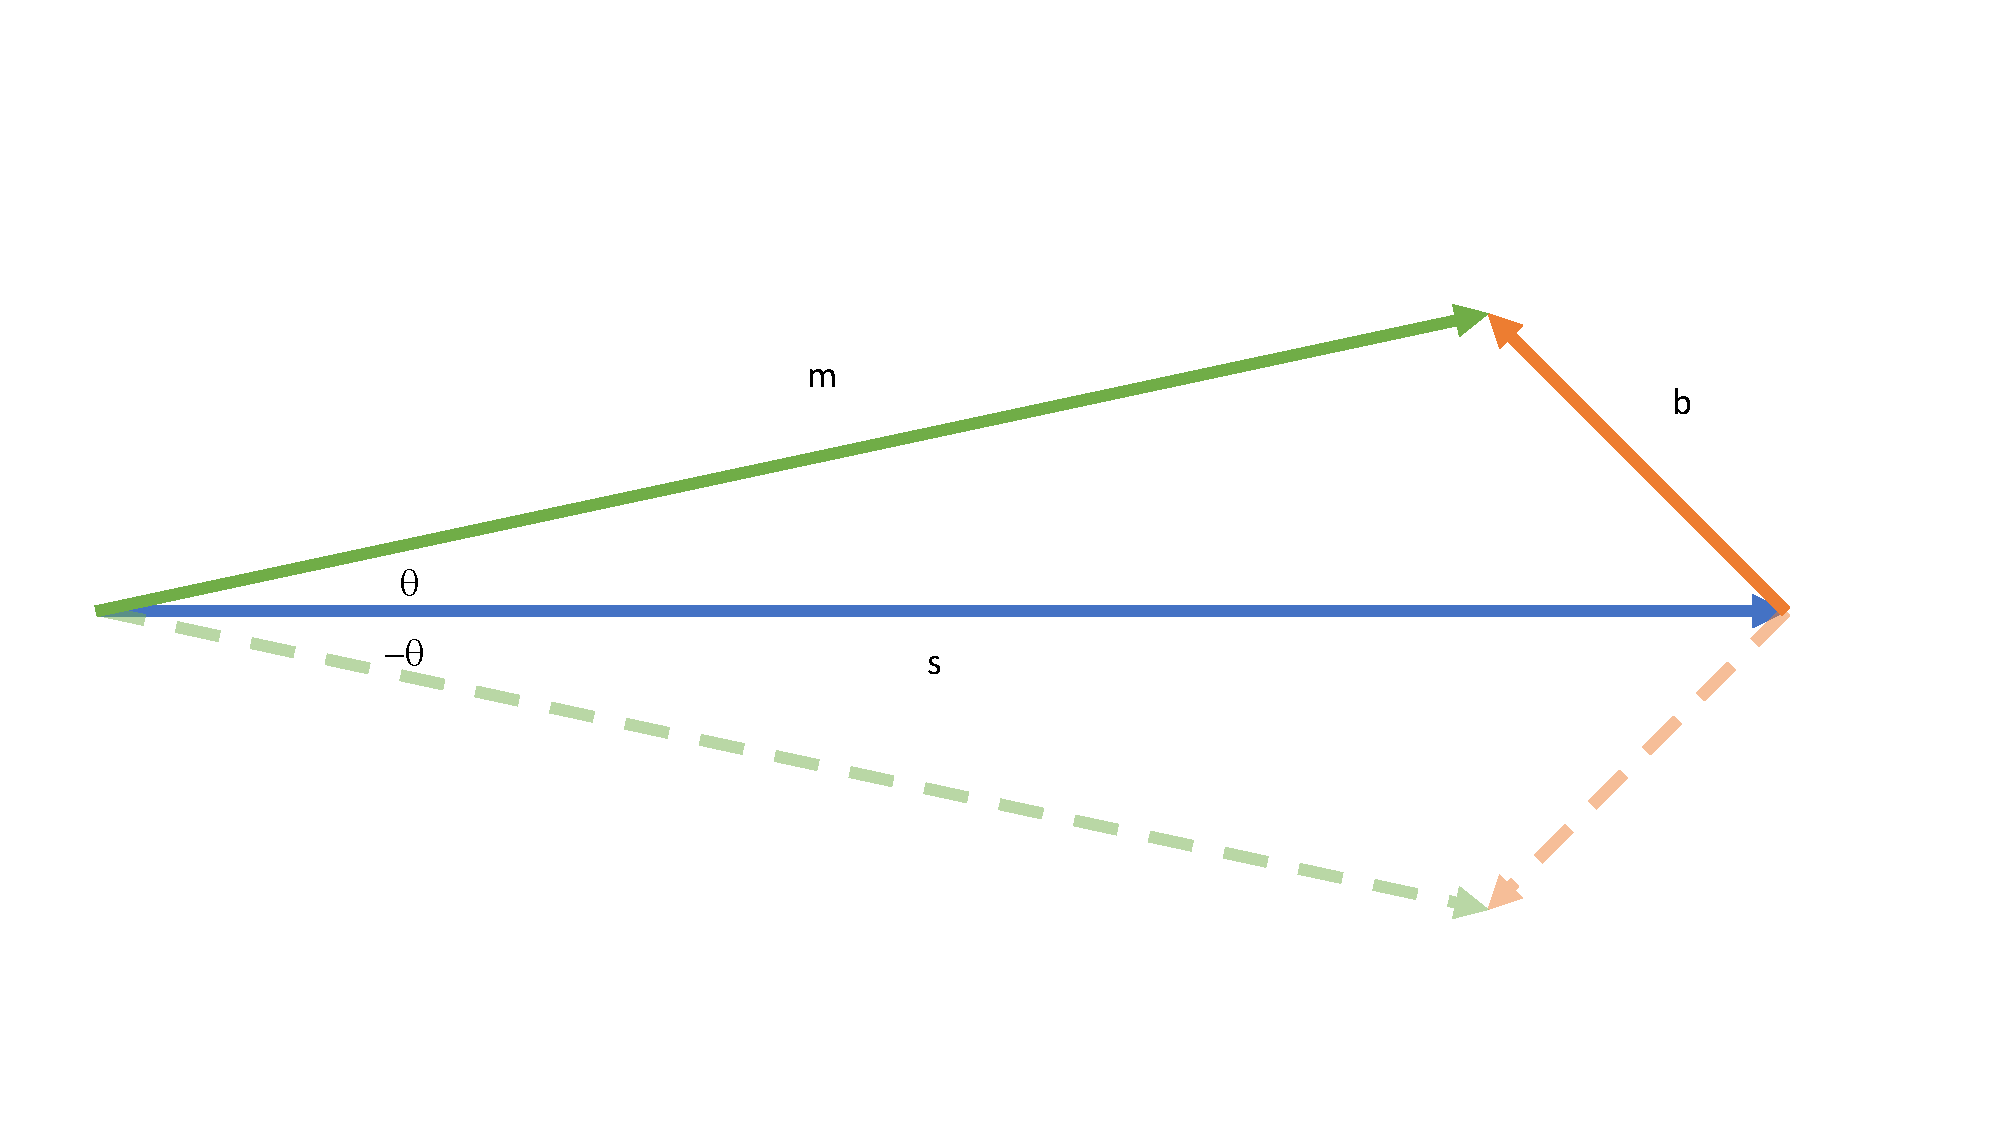
\includegraphics[width=1.0\textwidth]{figures/phasor_base.pdf}
\end{figure}

\par Our objective is to find the bearing correction that must be applied to the measured signal in order to arrive at the true cable signal.  This problem is most easily solved by considering the phasor representation.  Figure \ref{fig:phasor_base} shows the phasor representation for the same example model shown in Figure \ref{fig:phasor_base}.  In this representation, the correction angle, $\theta$ is readily obtained from the law of cosines.

\begin{equation} \label{eq:law_of_cos}
    \cos\left(\theta\right) = \frac{m^2 + s^2 - b^2}{2ms}
\end{equation}
But since $cos$ is an even function of its argument, we are unable to distinguish between solutions having postive and negative $\theta$.  So our solution becomes

\begin{equation} \label{eq:theta_solution}
\theta = \pm \cos^{-1}\left(\frac{m^2 + s^2 - b^2}{2ms}\right)
\end{equation}
where
\begin{align*}
        \theta &= \text{The angle between the measured and cable signals}\\
        s &= \text{cable signal amplitude.}\\
        b &= \text{background signal amplitude} \\
        m &= \text{measured signal amplitude} \\
\end{align*}



\subsection{Valid Solutions} \label{section:validity}
If the only information available from the system is the measured signal, there is no way to uniquely identify what the correction angle could be.  This is because there are infinitely many combinations of $s$, $b$, and $\theta$ that all generate exactly the same measured signal. We are not, however, free to pick any combination of $s$, $b$, and $\theta$.  The values we pick must be able to form a triangle in phasor space.  To get a feel for these constraints, we can rearrange eq. \ref{eq:law_of_cos} to the form
\begin{equation}
    b^2 = m^2 + s^2 - 2 m s \cos\left(\theta\right).
\end{equation}
In this form it is easy to see that, for fixes $m$ and $s$, the value of $b$ must be in the range

\begin{equation*}
      m^2 + s^2 - 2 m s \leq b ^ 2 \leq  m^2 + s^2 + 2 m s
\end{equation*}
or
\begin{equation} \label{eq:bounds}
      \left(m-s\right)^2 \leq b ^ 2 \leq \left(m + s\right)^2.  
\end{equation}
Any combination of $m$, $s$ and $b$ that satisfy equation \ref{eq:bounds} is a valid solution to the phasor triangle with a unique value for $\cos\left(\theta\right)$.  But again, since $\cos$ is an even function, we are only able to determine $\theta$ up to a sign.
    
\section{Statistical Treatment}
The last two sections have shown that if we only know the measured signal, there are infinitely many combinations of background and cable signal strengths that could have resulted in that measurement.  This, of course, assumed we had absolutely no knowledge of how big we expected the background and cable signals to be.  We now allow ourselves to apply additional constraints to our problem by specifying a range of plausible values for the background and cable signals.  In practice, these plausibility ranges are determined by conducting calibration runs of the pipe and cable we are working with.  In the calibration runs, we can take many measurements of the pipe with no cable attached.  These measurements will give us a sense of the range we can expect for the background signal.  Similarly, we can carefully set up a calibration run where we deliberately configure the system to have negligible background.  In this configuration, we can measure different cable attachments to get a sense of the range we can expect for the cable signal.  We can characterize these ranges as being statistical distributions with a given mean, $\mu$, and standard deviation, $\sigma$. There are any number of statistical distributions we could use, but here we select the gamma distribution.  Our primary motivation for selecting the Gamma distribution is that, like the amplitudes we are modeling, it is only defined for positive values.  We could have chosen any other distribution with this property, but the Gamma distribution is well understood and widely used. 

\par Based onWe use a monte-carlo simulation algorithm to estimate the distribution of the bearingOur procedure will then be as follows:

% \lstinputlisting[language=Python]{monte_car}


\begin{algorithm}[H]
\SetAlgoLined
\KwResult{Random samples drawn from distribution of bearing correction angles }
 $m \leftarrow$ input the measured signal amplitude\;
 $\mu_s \leftarrow$ input the cable signal mean\;
 $\sigma_s \leftarrow$ input the cable signal standard deviation\;
 $\mu_b \leftarrow$ input the background mean\;
 $\sigma_b \leftarrow$ input the background standard deviation\;
 
 
 \While{While condition}{
  instructions\;
  \eIf{condition}{
   instructions1\;
   instructions2\;
   }{
   instructions3\;
  }
 }
 \caption{How to write algorithms}
\end{algorithm}







\section{Bogus}
The density distribution for the gamma function is

\begin{equation} \label{eq:gamma_dist}
f\left(x\right) = \frac{1}{\Gamma\left(k\right)\phi^k}x^{k-1}e^{-\frac{x}{\phi}}
\end{equation}
where 
%$f$ is the probability density, $\Gamma$ is the Gamma function, $k$ is the shape parameter, and $\phi$ is the scale %parameter.
\begin{align*}
        f\left(x\right) &= \text{The probability density}\\
        \Gamma &= \text{The Gamma function}\\
        k &= \left(\frac{\mu}{\sigma}\right)^2 = \text{the shape parameter} \\
        \phi &= \frac{\sigma^2}{\mu} = \text{the scale parameter} \\
        \mu &= \frac{\sigma^2}{\mu} = \text{the mean} \\
        \sigma &= \frac{\sigma^2}{\mu} = \text{the standard deviation} \\
\end{align*}

\par  The approach we take to finding the 


\end{appendices}




%%% End document
\end{document}